\documentclass{beamer}

\usepackage{eecs}

\usepackage[all]{xy}
\usepackage{xmpmulti}
\usepackage{pdfpages}
\usepackage{fancyvrb}

\SaveVerb{bind}+>>=+
\SaveVerb{from}+<-+

\title[JavaScript DSLs]{Sunroof and a Blank Canvas:\\A tail of two DSLs}
\author[Andy Gill]{Andy Gill\\~\\with Jan Bracker (Sunroof) and Andrew Farmer (Blank Canvas)}
\institute{University of Kansas}
\date{July 8, 2014}

\begin{document}

\frame{\titlepage}

\begin{frame}[fragile]
\frametitle{Blank Canvas}
\Large
\begin{itemize}
\item library for simple graphics
\item Uses HTML5's \verb|<canvas>| capabilities as viewport
\item Javascript examples can be transliterated into Haskell    
\item Fast enough for basic animations
\end{itemize}
\begin{columns}
\begin{column}{0.45\textwidth}
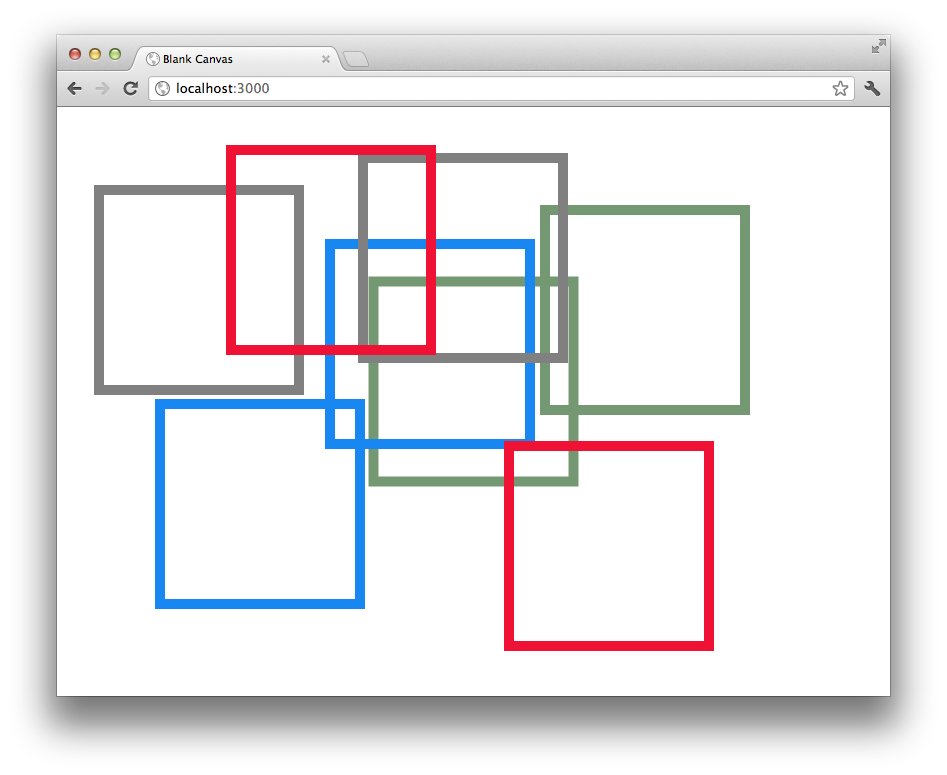
\includegraphics[width=150pt]{squares.png}
\end{column}
\begin{column}{0.55\textwidth}
\begin{codeblock}[0.6]
\footnotesize
\begin{verbatim}
...
translate (x,y)
beginPath()
moveTo(-100,-100)
lineTo(-100,100)
lineTo(100,100)
lineTo(100,-100)
closePath()
lineWidth 10
strokeStyle color
stroke()
...
\end{verbatim}
\end{codeblock}
\end{column}
\end{columns}
%\frameskip{}
%Why another image processing tool?
%\begin{itemize}
%\item Need a machine independent way of scripting up graphics in Haskell.
%\end{itemize}


\end{frame}

\begin{frame}[fragile]
\frametitle{Sunroof}
\large
\begin{itemize}
\item Deep embedding of the JavaScript syntax
\item Can write JavaScript in Haskell, access JavaScript APIs
\item CPS translation to supporting concurrency, when needed
\item The monadic bind translates into an assignment in JavaScript
\end{itemize}
\begin{codeblock}[0.75]
\footnotesize
\begin{verbatim}
currentTime :: JS t (JSNumber, JSNumber, JSNumber)
currentTime = do
  date <- newDate ()
  h <- date # getHours
  m <- date # getMinutes
  s <- date # getSeconds
  return (h, m, s)
\end{verbatim}
\end{codeblock}
\end{frame}

\begin{frame}[fragile]
\frametitle{First Sunroof Example: red line}
\Large



\begin{columns}
\begin{column}{0.40\textwidth}
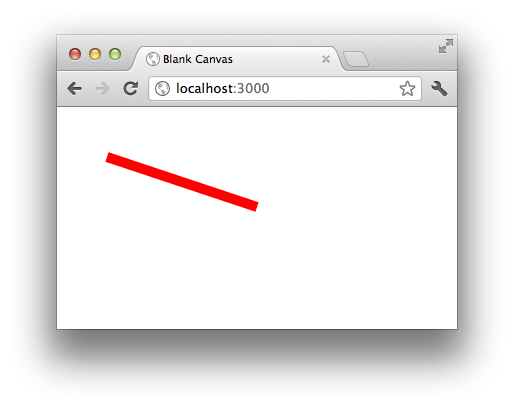
\includegraphics[width=150pt]{red-line.png}
\end{column}
\begin{column}{0.60\textwidth}
\begin{codeblock}[0.95]
\footnotesize
\begin{semiverbatim}
import Graphics.Blank
\uncover<2->{
main = blankCanvas 3000 \$ \\ context -> do\uncover<3->{
        send context \$ do\uncover<4->{
                moveTo(50,50)
                lineTo(200,100)
                lineWidth 10
                strokeStyle "red"
                stroke}}}
\end{semiverbatim}
\end{codeblock}
\end{column}
\end{columns}

\frameskip{}
\only<1>%
{First, include the {\tt Graphics.Blank} module.\vspace{0.58in}}
\only<2>%
{Second, main calls {\tt blankCanvas}, with two arguments:%
\begin{itemize}
\item The port (3000) to publish the application on; and
\item and what to do with canvas.
\end{itemize}
}
\only<3>%
{Third, we {\tt send} to the canvas a list of monadic commands.\vspace{0.38in}}
\only<4>%
{Finally, here are the commands to draw a {\color{red}red} line.\vspace{0.58in}}

\end{frame}

\begin{frame}[fragile]
\frametitle{Architecture of {\tt blank-canvas}}
\Large

\begin{tabular}{ccc}
\begin{minipage}[b]{.4\textwidth}
\begin{codeblock}[0.85]
\small
Your application:\\
\footnotesize ``please draw red line''
\end{codeblock}
\begin{codeblock*}[0.85]{{\tt blank-canvas}}
\tiny
Canvas commands for drawing pictures.
\end{codeblock*}
\begin{codeblock*}[0.85]{{\tt kansas-comet}}
\tiny
Comet pattern for pushing to client.
\end{codeblock*}
\begin{codeblock*}[0.85]{{\tt scotty}}
\tiny 
Support for RESTful APIs.
\end{codeblock*}
\begin{codeblock*}[0.85]{{\tt warp}}
\tiny
Receiving web requests from clients;
give back responses \& web pages.
\end{codeblock*}
\end{minipage}
    & ~~~$\Huge\Longleftrightarrow$ & \raisebox{-.3\height}{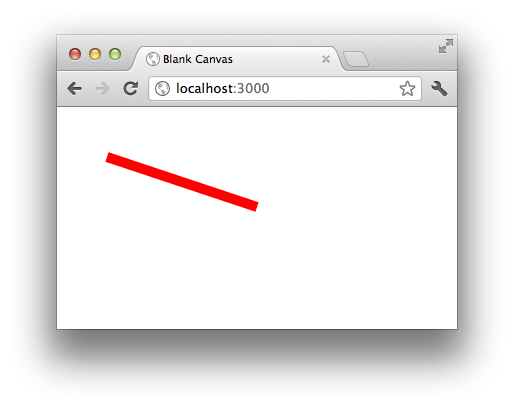
\includegraphics[width=150pt]{red-line.png}}\\
Software Stack & & Web Browser\\
\end{tabular}


\end{frame}

\begin{frame}[fragile]
\frametitle{Types in blank-canvas}
\large
\begin{codeblock}[0.99]
\begin{semiverbatim}
-- Create a web server. Run the given function with
-- a fresh Context each time our webpage is called.
blankCanvas :: Options -> (Context -> IO ()) -> IO ()

-- Sends a set of Canvas commands to the canvas. 
-- Attempts to common up as many commands as possible. 
-- A canvas command *may* return a result, which
-- will get passed back from the browser to the 
-- user, via the IO a.
send :: Context -> Canvas a -> IO a

-- Example of Canvas command
moveTo :: (Float, Float) -> Canvas ()
\end{semiverbatim}
\end{codeblock}        
\end{frame}




\begin{frame}[fragile]
\frametitle{Flow of Types}

\large
\begin{tabular}{rcrr}
        & \multicolumn{2}{c}{~~~~~{\tt Canvas a}}\\
        & \multicolumn{2}{c}{~~~~$\downarrow$}                    & Your Application\\
{\tt send ::}& \multicolumn{2}{c}{{\tt Context -> Canvas a -> IO a}}\\
        \cline{2-3}\noalign{\smallskip}
        & {\tt Context}~$\uparrow$      & $\downarrow$~{\tt IO~()}    & ~~~~{\tt  blank-canvas}\\
        \cline{2-3}\noalign{\smallskip}
        & \multicolumn{2}{c}{\tt IO ()}                                   & {\tt scotty}\\
\end{tabular}

\frameskip
\frameskip
\frameskip

\begin{itemize}
\item Drawings are constructed using the {\tt Canvas} monad
\item {\tt send} pushes a Canvas drawing to the screen
\item No way to get from inside the {\tt Canvas} monad
to the {\tt IO} monad
\item Hence, programs are written in {\tt IO}, with
islands of {\tt Canvas} drawing rendered via {\tt send}.
\item {\tt Canvas} results are returned to {\tt IO} via {\tt send}.
\end{itemize}        

\end{frame}



\begin{frame}[fragile]
\frametitle{From: {\tt http://www.html5canvastutorials.com/}}

\begin{codeblock}[0.8]
\tiny
\begin{semiverbatim}
<!DOCTYPE HTML>
<html>
  <head>
    <style>
      body \{
        margin: 0px;
        padding: 0px;
      \}
      #myCanvas \{
        border: 1px solid #9C9898;
      \}
    </style>
    <script>
      window.onload = function() \{
        var canvas = document.getElementById("myCanvas");
        var context = canvas.getContext("2d");

        \alert{context.moveTo(100, 150);
        context.lineTo(450, 50);
        context.stroke();}
      \};

    </script>
  </head>
  <body>
    <canvas id="myCanvas" width="578" height="200"\ \!\!\!></canvas>
  </body>
</html>
\end{semiverbatim}
\end{codeblock}
\end{frame}

\begin{frame}[fragile]
\frametitle{Example of Javascript to Haskell Transliteration}

\begin{columns}
\begin{column}{0.50\textwidth}
\begin{codeblock*}[0.85]{Javascript}
\begin{verbatim}
context.moveTo(100, 150);
context.lineTo(450, 50);
context.stroke();
\end{verbatim}
\end{codeblock*}
\end{column}

\pause{}
\begin{column}{0.50\textwidth}
\begin{codeblock*}[0.65]{Haskell}
\begin{verbatim}
send context $ do
   moveTo(100, 150)
   lineTo(450, 50)
   stroke()
\end{verbatim}
\end{codeblock*}
\end{column}

\end{columns}

\frameskip
\frameskip
\frameskip

\pause{}

\centering
\begin{codeblock*}[0.6]{Types in {\tt blank-canvas}}
\begin{verbatim}
moveTo :: (Float,Float) -> Canvas ()
lineTo :: (Float,Float) -> Canvas ()
stroke :: ()            -> Canvas ()

send :: Context -> Canvas a -> IO a
\end{verbatim}
\end{codeblock*}

\end{frame}        
        
\begin{frame}[fragile]
\frametitle{Supported Canvas Commands}

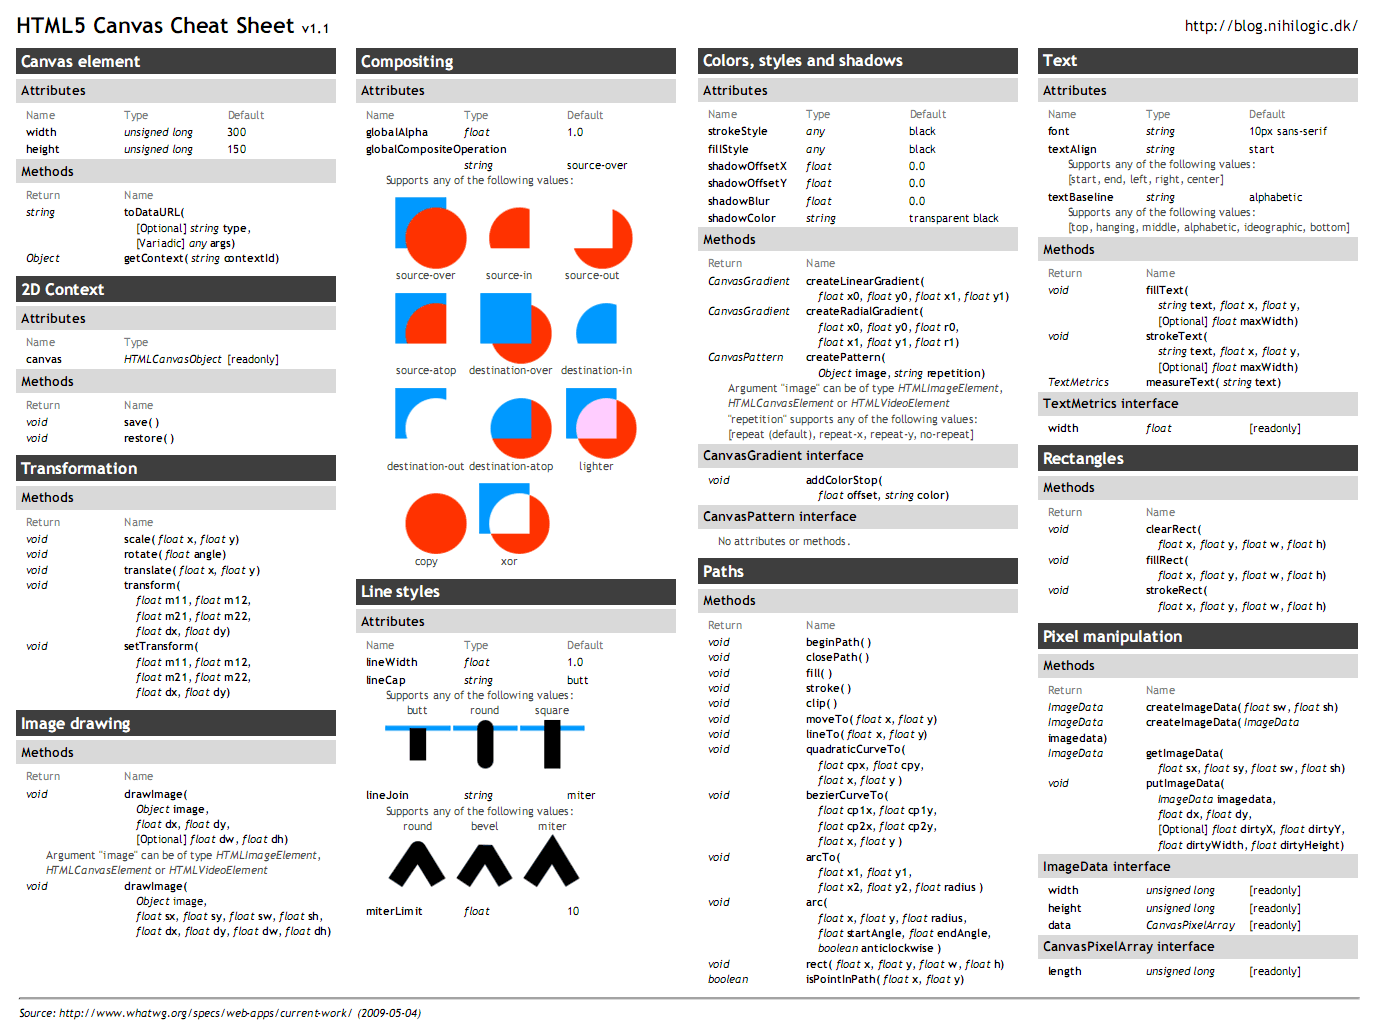
\includegraphics[width=.95\textwidth]{HTML5_Canvas_Cheat_Sheet.png}

\end{frame}

\begin{frame}[fragile]
\frametitle{Animation}

\Large
Animation is simply a matter of sending draw commands fast enough to the
browser window.

\begin{codeblock}[0.9]
\footnotesize
\begin{verbatim}
module Main where

import Graphics.Blank

main = blankCanvas 3000 $ \ context -> loop context (0 :: Float)

loop context n = do
        send context $ do
                -- clear the canvas
                ...
                -- draw the square
                ...
                
        loop context (n + 0.01)
\end{verbatim}
\end{codeblock}

\end{frame}

\begin{frame}[fragile]
\frametitle{Rotating Square}

\begin{columns}
\begin{column}{0.3\textwidth}
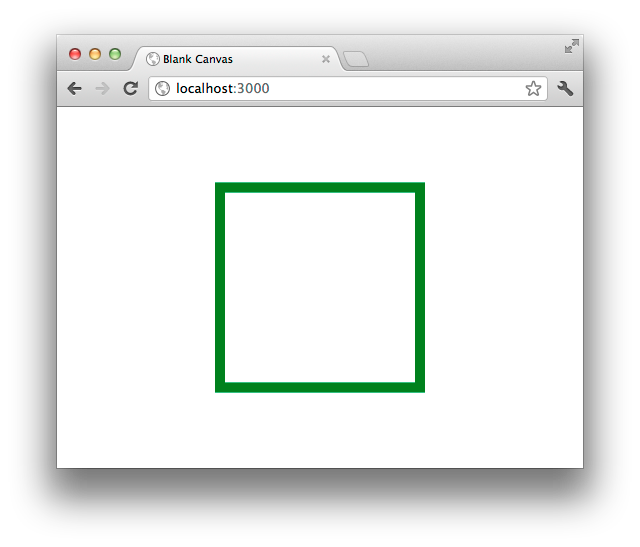
\includegraphics[trim = 25mm 30mm 25mm 25mm, clip, width=90pt]{1.png}\\
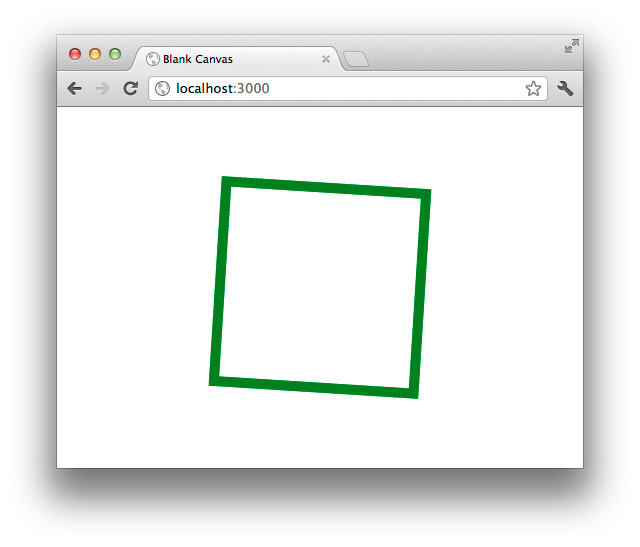
\includegraphics[trim = 25mm 30mm 25mm 25mm, clip, width=90pt]{3.png}\\
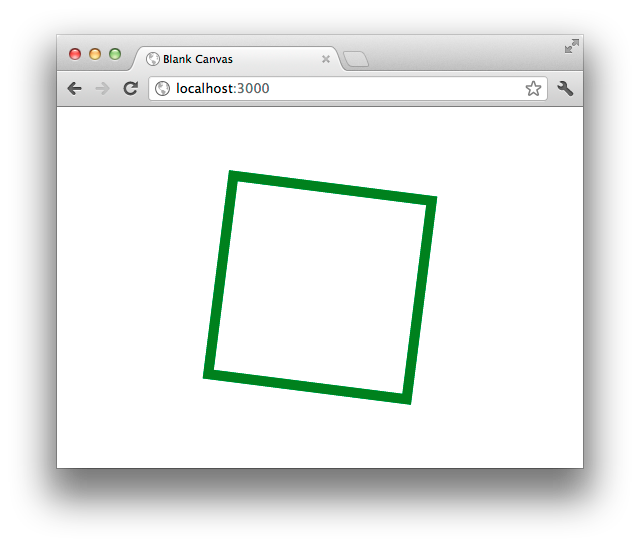
\includegraphics[trim = 25mm 30mm 25mm 25mm, clip, width=90pt]{5.png}
\end{column}
\begin{column}{0.7\textwidth}
\begin{codeblock}[0.8]
\tiny
\begin{semiverbatim}
loop context n = do
    send context \$ do
        clearRect (0,0,width context,height context)
        beginPath()
        save()
        translate (width context / 2,height context / 2)
        rotate (pi * n)
        beginPath()
        moveTo(-100,-100)
        lineTo(-100,100)
        lineTo(100,100)
        lineTo(100,-100)
        closePath()
        lineWidth 10
        strokeStyle "green"
        stroke()
        restore()
    threadDelay (20 * 1000) 
    loop context (n + 0.01)
\end{semiverbatim}
\end{codeblock}
\end{column}
\end{columns}


\end{frame}


\begin{frame}[fragile]
\frametitle{Explaining the drawing of the square}

\tiny

\begin{columns}[t]
\begin{column}{0.5\textwidth}

\begin{codeblock}[0.9]
\begin{semiverbatim}
clearRect (0,0,width context,height context)
beginPath()
\end{semiverbatim}
\end{codeblock}

\begin{codeblock}[0.9]
\begin{semiverbatim}
save()
\end{semiverbatim}
\end{codeblock}

\begin{codeblock}[0.9]
\begin{semiverbatim}
translate (width context / 2,height context / 2)
rotate (pi * n)
\end{semiverbatim}
\end{codeblock}

\begin{codeblock}[0.9]
\begin{semiverbatim}
beginPath()
moveTo(-100,-100)
lineTo(-100,100)
lineTo(100,100)
lineTo(100,-100)
closePath()
lineWidth 10
strokeStyle "green"
stroke()
\end{semiverbatim}
\end{codeblock}

\begin{codeblock}[0.9]
\begin{semiverbatim}
restore()
\end{semiverbatim}
\end{codeblock}

\end{column}
\begin{column}{0.4\textwidth}

\vskip 10pt
\noindent
Clear the screen.\\
({\tt beginPath()} is needed for line drawings.)

\vskip 20pt
\noindent
Save the state of the canvas. This is good practice.


\vskip 20pt
\noindent
These translations are applied to all coordinates.

\vskip 20pt
\noindent
At last we can draw the square!  Notice how we draw
a 200x200 square, centered on (0,0), 
and rely on the previous translations
to give us rotation.

\vskip 55pt
\noindent
Restore the state of the canvas.\\
This undoes the translations.

\end{column}
\end{columns} 
\end{frame}

\begin{frame}[fragile]
\frametitle{Interaction}

So far, everything has about been {\em sending\/} commands JavaScript.\\
~\\

There are two types of browser${}\rightarrow{}$application interaction.\\
~\\

{\bf The HTML canvas, if asked, can listen for events.}
\begin{itemize}
\item Examples are \verb|mousedown| and \verb|mousemove|.
\item We need to send the events to the Haskell program.
\item We handle events using a STM Queue.
\end{itemize}
~\\
{\bf We can also {\em query\/} the JavaScript state inside \verb|Canvas|.}
\begin{itemize}
\item For example, is a point inside a path?
\end{itemize}
\begin{codeblock}[0.8]
\begin{semiverbatim}
isPointInPath :: (Float, Float) -> Canvas Bool
\end{semiverbatim}
\end{codeblock}
~\\
\begin{itemize}
\item Question: How do we get the boolean back to Haskell?
\end{itemize}
\end{frame}


\begin{frame}[fragile]
\frametitle{The Canvas Monad}

{\tt Canvas} provides a deep DSL. This allows for certain optimizations,
specifically we try bundle together as much as possible when
sending drawing commands to the browser.

\begin{codeblock}[0.9]
\tiny
\begin{verbatim}

data Canvas :: * -> * where
        Method  :: Method                              -> Canvas ()     -- <context>.<method>
        Command :: Command                             -> Canvas ()     -- <command>
        Query   :: Query a                             -> Canvas a
        ...
        Bind    :: Canvas a -> (a -> Canvas b)         -> Canvas b
        Return  :: a                                   -> Canvas a

instance Monad Canvas where
        return = Return
        (>>=) = Bind

data Method
        = Arc (Float,Float,Float,Float,Float,Bool)
        | ArcTo (Float,Float,Float,Float,Float)
        | BeginPath
        | BezierCurveTo (Float,Float,Float,Float,Float,Float)
        | forall image . Image image => DrawImage (image,[Float])
        ...

data Query :: * -> * where
        IsPointInPath        :: (Float,Float)             -> Query Bool
        ...
\end{verbatim}

\end{codeblock}

\end{frame}

\begin{frame}[fragile]
\frametitle{GADTs to the rescue!}

We interpret the \verb|Canvas| monad, collecting JavaScript, punctuating at queries.

\begin{codeblock}[1]
\tiny
\begin{semiverbatim}
send :: DeviceContext -> Canvas a -> IO a
send cxt commands = send' (deviceCanvasContext cxt) commands id 
 where
  send' :: CanvasContext -> Canvas a -> (String -> String) -> IO a
  send' c (\alert{Bind} (\alert{Return} a) k)    cmds = send' c (k a) cmds
  send' c (\alert{Bind} (\alert{Bind} m k1) k2)  cmds = send' c (Bind m (\ r -> Bind (k1 r) k2)) cmds
  send' c (Bind (Method cmd) k) cmds = send' c (k ()) (cmds . ((showJS c ++ ".") ++) . shows cmd . (";" ++))
  send' c (Bind (Command cmd) k) cmds = send' c (k ()) (cmds . shows cmd . (";" ++))
  send' c (Bind (\alert{Query} query) k) cmds = do
      uq <- atomically \$ getUniq
      -- The query function returns a function takes the unique port number of the reply.
      sendToCanvas cxt (cmds . ((show query ++ "(" ++ show uq ++ "," ++ showJS c ++ ");") ++))
      v <- KC.getReply (theComet cxt) uq
      case parse (parseQueryResult query) v of
        Error msg -> fail msg
        Success a -> do
                send' c (k a) id
  ...
  send' _ (Return a)           cmds = do
      sendToCanvas cxt cmds
      return a
  send' c cmd                  cmds = send' c (Bind cmd Return) cmds

\alert{parseQueryResult} :: Query a -> Value -> Parser a
...
\end{semiverbatim}

\end{codeblock}

\end{frame}

\begin{frame}[fragile]{Sunroof binds do not return to Haskell}

\begin{itemize}
\item Can we avoid returning to Haskell? Yes. 
\item Sunroof is based on this idea.
\end{itemize}

~\\
~\\
JavaScript:

\begin{codeblock}[0.4]
\tiny
\begin{verbatim}
var name = prompt("Your name?");
alert("Your name: " + name);
\end{verbatim}
\end{codeblock}

~\\
Sunroof:

\begin{codeblock}[0.4]
\tiny
\begin{verbatim}
do name <- prompt "Your name?"
   alert ("Your name: " <> name)

prompt :: JSString -> JS JSString
alert  :: JSString -> JS ()
\end{verbatim}
\end{codeblock}

\end{frame}



\begin{frame}[fragile]{Key idea - normalize the constraints}

\begin{columns}
\begin{column}{0.45\textwidth}

\begin{codeblock}[0.8]
\tiny
\begin{verbatim}
(>>=) :: JS a -> (a -> JS b) -> JS b
\end{verbatim}
\end{codeblock}


\begin{itemize}
\item We need to know that 'a' is a JavaScript type.
\item {\bf How do we constrain it?} Normalize and reify the monad!
\end{itemize}

\end{column}

\begin{column}{0.55\textwidth}

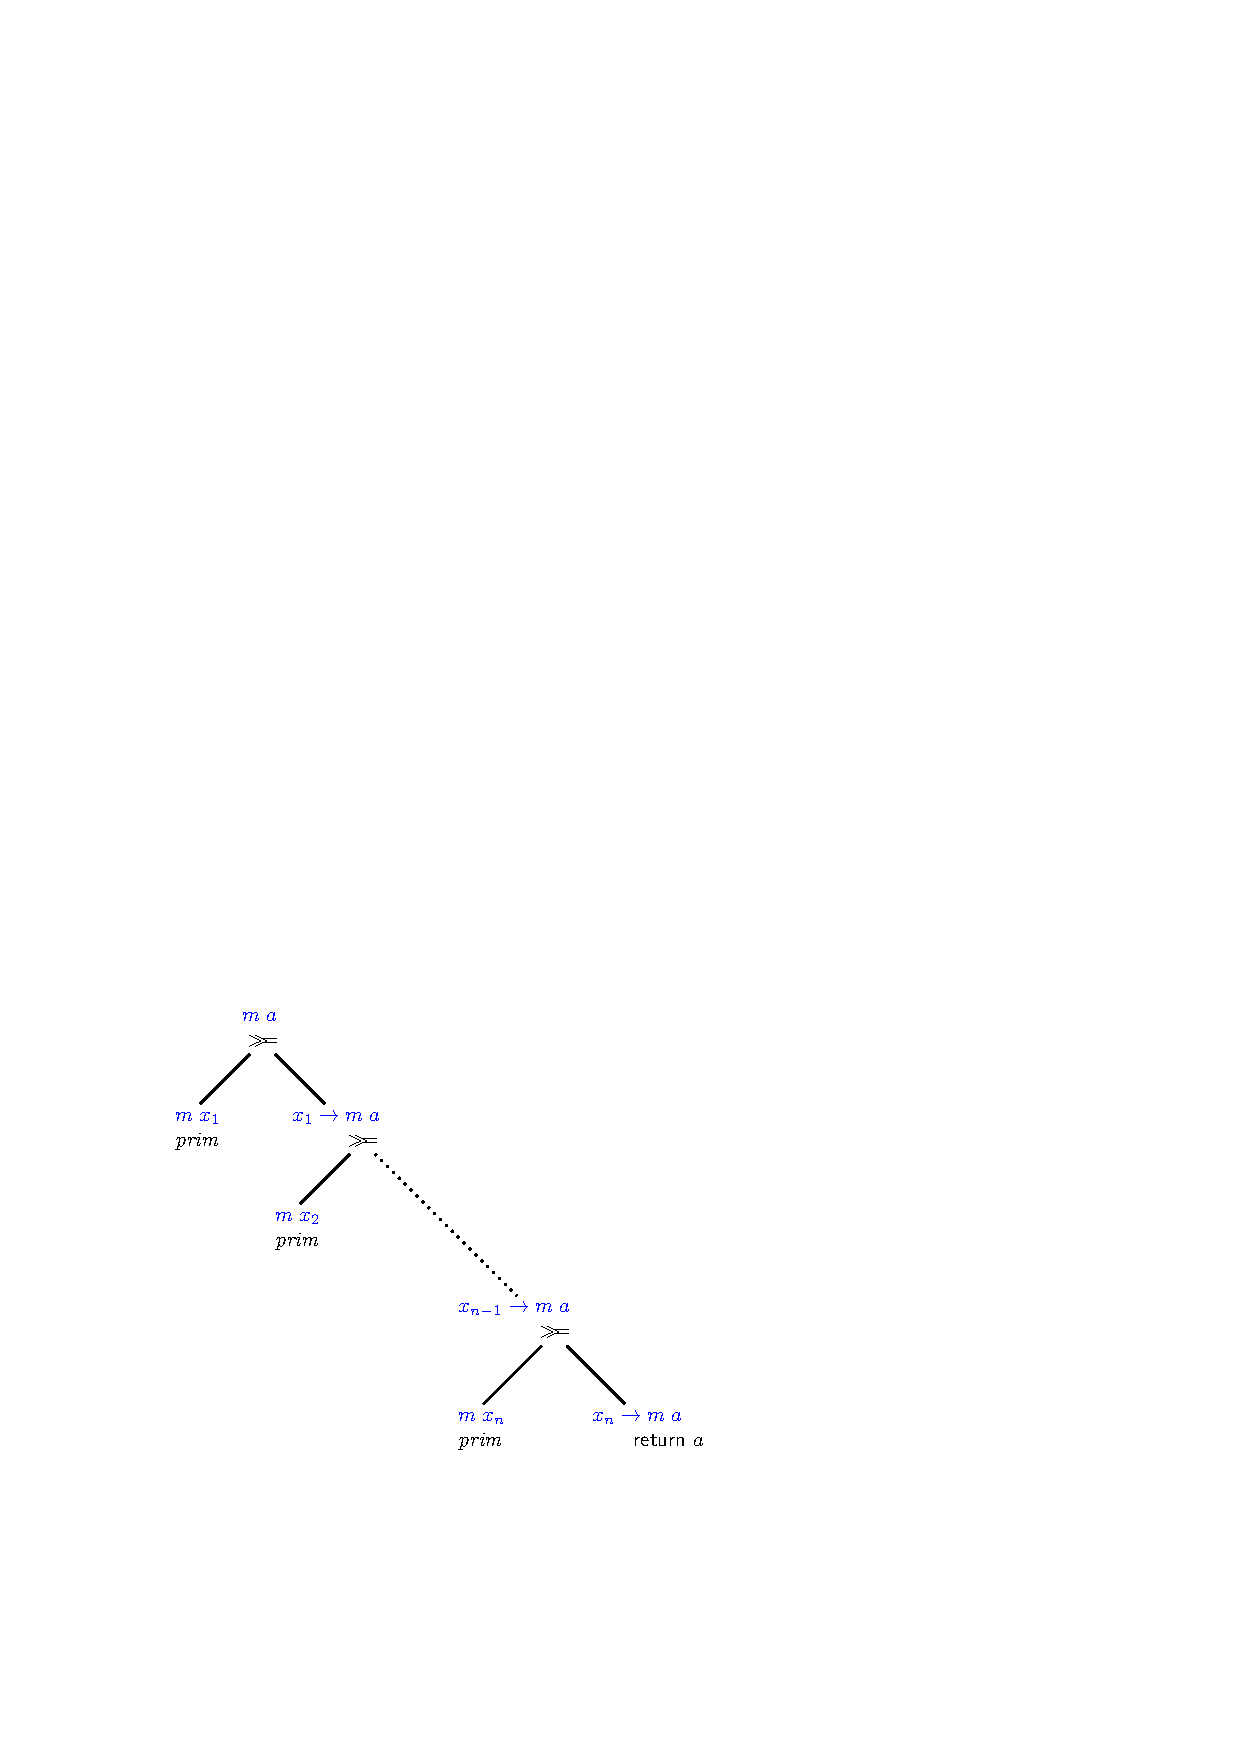
\includegraphics[width=150pt]{MonadNormalForm.pdf}

\end{column}
\end{columns}

~\\
~\\
See: The Constrained-Monad Problem, ICFP'13, Sculthorpe, et. al.\ for details.


\end{frame}

\begin{frame}[fragile]{Threading Models}

Actually the `JS` data type has another type parameter `t`:

\begin{codeblock}[0.15]
\small
\begin{verbatim}
JS t a
\end{verbatim}
\end{codeblock}

\begin{itemize}
\item `t` determines the threading model used
\item `t` can either be \verb`A` or \verb`B`
\end{itemize}

\begin{columns}
\begin{column}{0.5\textwidth}
Model A: Atomic
\begin{itemize}
\item The JavaScript threading model
\item Callback centric
\item One thread with event loop
\item Executed code in loop is uninterruptible
\end{itemize}
\end{column}
\begin{column}{0.5\textwidth}
Model B: Blocking

\begin{itemize}
\item Adds cooperative concurrency to Sunroof
\item Offers abstractions known from Haskell: 
\end{itemize}

\begin{codeblock}[0.6]
\begin{verbatim}
forkJS :: JS B () -> JS t ()
yield :: JS B ()
\end{verbatim}
\end{codeblock}

~\\
Also \verb|JSMVar| and \verb|JSChan|.

\begin{itemize}
\item Implemented through translation of continuations to JavaScript
\end{itemize}

\end{column}
\end{columns}

\end{frame}

\begin{frame}[fragile]{Functions}

\begin{codeblock}[0.8]
\begin{verbatim}
function   :: (...) => (a -> JS A r) 
                    -> JS t (JSFunction a r)
apply,($$) :: (...) => JSFunction a r 
                    -> a -> JS t r
\end{verbatim}
\end{codeblock}


\begin{codeblock}[0.8]
\begin{verbatim}
square :: JS t (JSFunction JSNumber JSNumber)
square = function $ \x -> return (x * x)
\end{verbatim}
\end{codeblock}

\begin{codeblock}[0.8]
\begin{verbatim}
jsCode = do
  sqr <- square   -- Create / Bind
  n <- sqr $$ 2  -- Use
  ...
\end{verbatim}
\end{codeblock}
\end{frame}

\begin{frame}[fragile]{Continuations}

\begin{itemize}
\item Continuations needed for second threading model
\item \verb`JS`-monad is a continuation monad
\item We have access to the underlying continuations in JavaScript
\end{itemize}


\begin{codeblock}[0.9]
\begin{verbatim}
continuation   :: (...) => (a -> JS B ()) 
                        -> JS t (JSContinuation a)
goto           :: (...) => JSContinuation a
                        -> a -> JS t b
\end{verbatim}
\end{codeblock}

We even have our friend, call/cc.

\begin{codeblock}[0.9]
\begin{verbatim}
callcc :: (...) => (JSContinuation a -> JS B a)
                -> JS B a
\end{verbatim}
\end{codeblock}

\end{frame}


\begin{frame}[fragile]{So how well does it all work?}
        
\begin{itemize}
\item The types are quite complex
\item Wrote a number of applications (calculator; grader program)
\item Control flow is the {\bf pain point}
\end{itemize}                

\end{frame}

\end{document}
